\subsection{Kernel configuration}

\begin{frame}
  \frametitle{Kernel configuration and build system}
  \begin{itemize}
  \item The kernel configuration and build system is based on multiple
    Makefiles
  \item One only interacts with the main \kpath{Makefile}, present at
    the {\bf top directory} of the kernel source tree
  \item Interaction takes place
    \begin{itemize}
    \item using the \code{make} tool, which parses the Makefile
    \item through various {\bf targets}, defining which action should
      be done (configuration, compilation, installation, etc.). Run
      \code{make help} to see all available targets.
    \end{itemize}
  \item Example
    \begin{itemize}
    \item \code{cd linux-3.6.x/}
    \item \code{make <target>}
    \end{itemize}
  \end{itemize}
\end{frame}

\begin{frame}
  \frametitle{Kernel configuration (1)}
  \begin{itemize}
  \item The kernel contains thousands of device drivers, filesystem
    drivers, network protocols and other configurable items
  \item Thousands of options are available, that are used to
    selectively compile parts of the kernel source code
  \item The kernel configuration is the process of defining the set of
    options with which you want your kernel to be compiled
  \item The set of options depends
    \begin{itemize}
    \item On your hardware (for device drivers, etc.)
    \item On the capabilities you would like to give to your kernel
      (network capabilities, filesystems, real-time, etc.)
    \end{itemize}
  \end{itemize}
\end{frame}

\begin{frame}
  \frametitle{Kernel configuration (2)}
  \begin{itemize}
  \item The configuration is stored in the \code{.config} file at the
    root of kernel sources
    \begin{itemize}
    \item Simple text file, \code{key=value} style
    \end{itemize}
  \item As options have dependencies, typically never edited by hand,
    but through graphical or text interfaces:
    \begin{itemize}
    \item \code{make xconfig}, \code{make gconfig} (graphical)
    \item \code{make menuconfig}, \code{make nconfig} (text)
    \item You can switch from one to another, they all load/save the
      same \code{.config} file, and show the same set of options
    \end{itemize}
  \item To modify a kernel in a GNU/Linux distribution: the
    configuration files are usually released in \code{/boot/},
    together with kernel images: \code{/boot/config-3.2.0-31-generic}
  \end{itemize}
\end{frame}

\begin{frame}
  \frametitle{Kernel or module?}
  \begin{itemize}
  \item The {\bf kernel image} is a {\bf single file}, resulting from
    the linking of all object files that correspond to features
    enabled in the configuration
    \begin{itemize}
    \item This is the file that gets loaded in memory by the
      bootloader
    \item All included features are therefore available as soon as the
      kernel starts, at a time where no filesystem exists
    \end{itemize}
  \item Some features (device drivers, filesystems, etc.) can however
    be compiled as {\bf modules}
    \begin{itemize}
    \item These are {\em plugins} that can be loaded/unloaded dynamically to
      add/remove features to the kernel
    \item Each {\bf module is stored as a separate file in the
        filesystem}, and therefore access to a filesystem is mandatory
      to use modules
    \item This is not possible in the early boot procedure of the
      kernel, because no filesystem is available
    \end{itemize}
  \end{itemize}
\end{frame}

\begin{frame}
  \frametitle{Kernel option types}
  There are different types of options
  \begin{itemize}
  \item \code{bool} options, they are either
    \begin{itemize}
    \item {\em true} (to include the feature in the kernel) or
    \item {\em false} (to exclude the feature from the kernel)
    \end{itemize}
  \item \code{tristate} options, they are either
    \begin{itemize}
    \item {\em true} (to include the feature in the kernel image) or
    \item {\em module} (to include the feature as a kernel module) or
    \item {\em false} (to exclude the feature)
    \end{itemize}
  \item \code{int} options, to specify integer values
  \item \code{hex} options, to specify hexadecimal values
  \item \code{string} options, to specify string values
  \end{itemize}
\end{frame}

\begin{frame}
  \frametitle{Kernel option dependencies}
  \begin{itemize}
  \item There are dependencies between kernel options
  \item For example, enabling a network driver requires the network
    stack to be enabled
  \item Two types of dependencies
    \begin{itemize}
    \item \code{depends on} dependencies. In this case, option A that
      depends on option B is not visible until option B is enabled
    \item \code{select} dependencies. In this case, with option A
      depending on option B, when option A is enabled, option B is
      automatically enabled
    \end{itemize}
  \item \code{make xconfig} allows to see all options, even the ones
    that cannot be selected because of missing dependencies. In this
    case, they are displayed in gray.
  \end{itemize}
\end{frame}

\begin{frame}
  \frametitle{make xconfig}
  \code{make xconfig}
  \begin{itemize}
  \item The most common graphical interface to configure the kernel.
  \item Make sure you read\\
    \code{help ->  introduction: useful options!}
  \item File browser: easier to load configuration files
  \item Search interface to look for parameters
  \item Required Debian / Ubuntu packages: \code{libqt4-dev} \code{g++}
  \end{itemize}
\end{frame}

\begin{frame}
  \frametitle{make xconfig screenshot}
  \begin{center}
    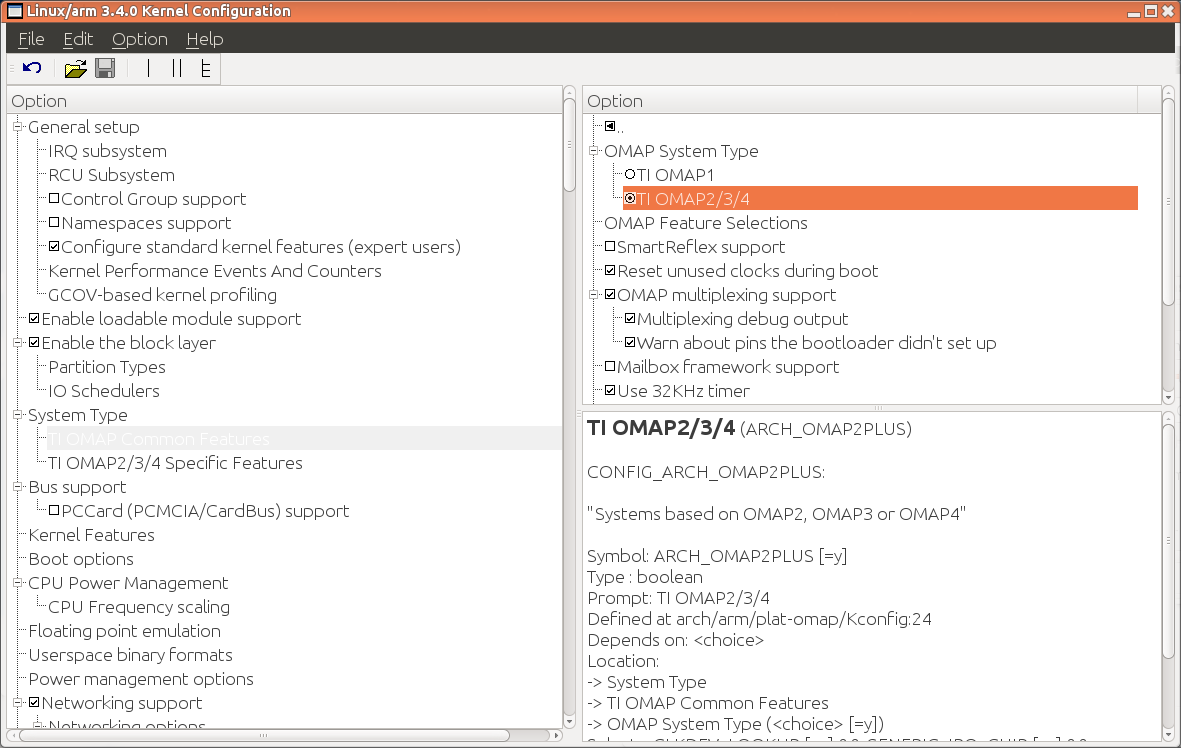
\includegraphics[width=\textwidth]{slides/sysdev-linux-intro-configuration/xconfig-screenshot.png}
  \end{center}
\end{frame}

\begin{frame}
  \frametitle{make xconfig search interface}

  Looks for a keyword in the parameter name. Allows to select or
  unselect found parameters.

  \begin{center}
    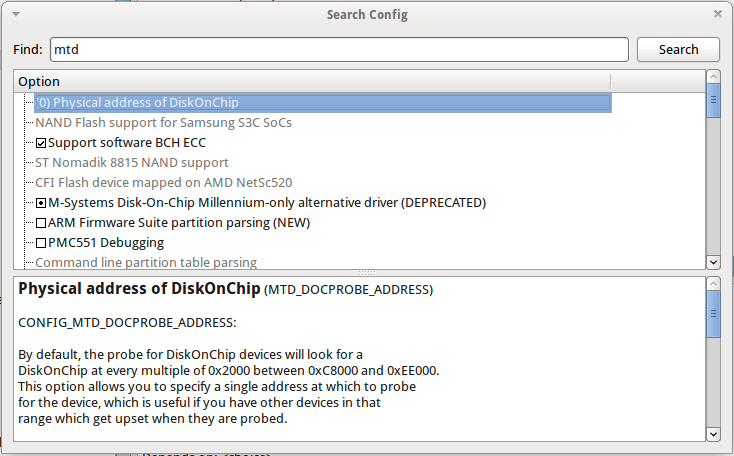
\includegraphics[width=0.9\textwidth]{slides/sysdev-linux-intro-configuration/xconfig-search.png}
  \end{center}
\end{frame}

\begin{frame}
\frametitle{Kernel configuration options}
  \begin{center}
    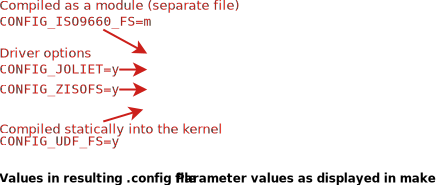
\includegraphics[width=\textwidth]{slides/sysdev-linux-intro-configuration/xconfig-iso-example.pdf}
  \end{center}
\end{frame}

\begin{frame}[fragile]
  \frametitle{Corresponding .config file excerpt}
  Options are grouped by sections and are prefixed with
  \code{CONFIG_}.
\small
\begin{verbatim}
#
# CD-ROM/DVD Filesystems
#
CONFIG_ISO9660_FS=m
CONFIG_JOLIET=y
CONFIG_ZISOFS=y
CONFIG_UDF_FS=y
CONFIG_UDF_NLS=y

#
# DOS/FAT/NT Filesystems
#
# CONFIG_MSDOS_FS is not set
# CONFIG_VFAT_FS is not set
CONFIG_NTFS_FS=m
# CONFIG_NTFS_DEBUG is not set
CONFIG_NTFS_RW=y
\end{verbatim}
\end{frame}

\begin{frame}
  \frametitle{make gconfig}
  \begin{columns}
    \column{0.5\textwidth}
    \code{make gconfig}
    \begin{itemize}
      \item {\em GTK} based graphical configuration interface. Functionality
            similar to that of make \code{xconfig}.
      \item Just lacking a search functionality.
      \item Required Debian packages: \code{libglade2-dev}
    \end{itemize}
    \column{0.5\textwidth}
    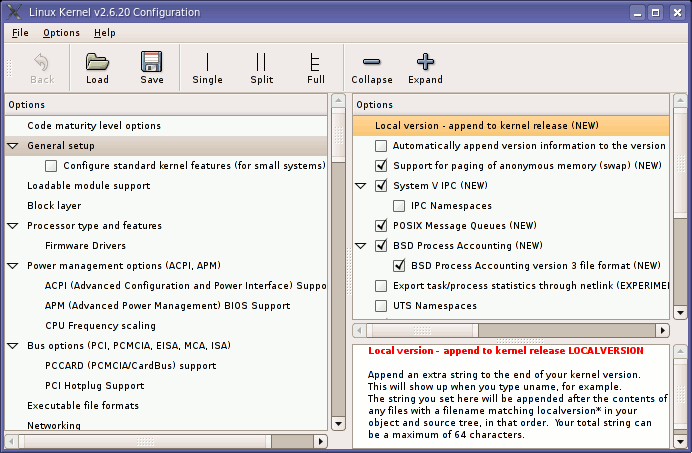
\includegraphics[width=0.9\textwidth]{slides/sysdev-linux-intro-configuration/gconfig-screenshot.png}
  \end{columns}
\end{frame}

\begin{frame}
  \frametitle{make menuconfig}
  \begin{columns}
    \column{0.5\textwidth}
    \code{make menuconfig}
    \begin{itemize}
      \item Useful when no graphics are available. Pretty convenient too!
      \item Same interface found in other tools: BusyBox, Buildroot...
      \item Required Debian packages: \code{libncurses-dev}
    \end{itemize}
    \column{0.5\textwidth}
    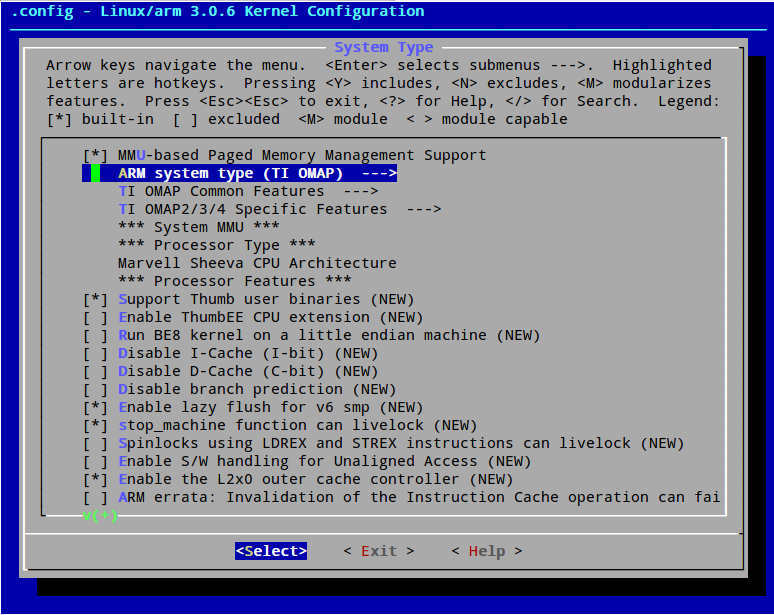
\includegraphics[width=0.9\textwidth]{slides/sysdev-linux-intro-configuration/menuconfig-screenshot.png}
  \end{columns}
\end{frame}

\begin{frame}
  \frametitle{make nconfig}
  \begin{columns}
    \column{0.5\textwidth}
    \code{make nconfig}
    \begin{itemize}
      \item A newer, similar text interface
      \item More user friendly (for example, easier to access help information).
      \item Required Debian packages: \code{libncurses-dev}
    \end{itemize}
    \column{0.5\textwidth}
    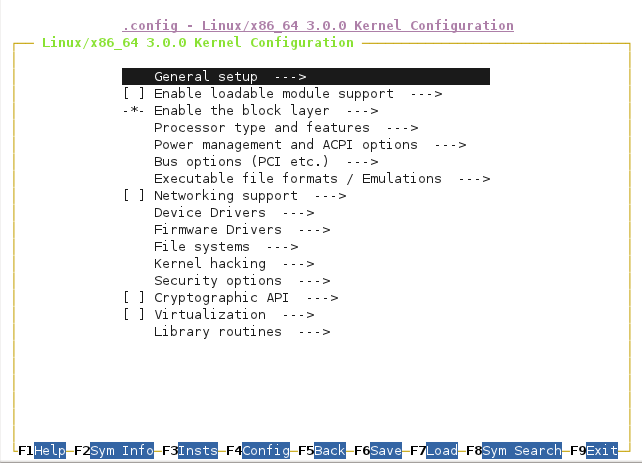
\includegraphics[width=0.9\textwidth]{slides/sysdev-linux-intro-configuration/nconfig-screenshot.png}
  \end{columns}
\end{frame}

\begin{frame}
  \frametitle{make oldconfig}
  \code{make oldconfig}
  \begin{itemize}
  \item Needed very often!
  \item Useful to upgrade a \code{.config} file from an earlier kernel release
  \item Issues warnings for configuration parameters that no longer
    exist in the new kernel.
  \item Asks for values for new parameters (while \code{xconfig}
    and \code{menuconfig} silently set default values for new
    parameters).
  \end{itemize}
  If you edit a \code{.config} file by hand, it's strongly recommended
  to run \code{make oldconfig} afterwards!
\end{frame}

\begin{frame}
  \frametitle{Undoing configuration changes}
  A frequent problem:
  \begin{itemize}
  \item After changing several kernel configuration settings, your
    kernel no longer works.
  \item If you don't remember all the changes you made,
    you can get back to your previous configuration:\\
    \code{$ cp .config.old .config}
  \item All the configuration interfaces of the kernel
    (\code{xconfig}, \code{menuconfig}, \code{oldconfig}...) keep
    this \code{.config.old} backup copy.
  \end{itemize}
\end{frame}

\begin{frame}
  \frametitle{Configuration per architecture}
  \begin{itemize}
  \item The set of configuration options is architecture dependent
    \begin{itemize}
    \item Some configuration options are very architecture-specific
    \item Most of the configuration options (global kernel options,
      network subsystem, filesystems, most of the device drivers) are
      visible in all architectures.
    \end{itemize}
  \item By default, the kernel build system assumes that the kernel is
    being built for the host architecture, i.e. native compilation
  \item The architecture is not defined inside the configuration, but
    at a higher level
  \item We will see later how to override this behaviour, to allow the
    configuration of kernels for a different architecture
  \end{itemize}
\end{frame}
